\documentclass[8pt, hyperref={pdfpagelabels=false}]{beamer}
\let\Tiny=\tiny
\usepackage[T2A]{fontenc}
\usepackage{pscyr}
\usepackage[russian]{babel}
\usepackage[utf8]{inputenc}
\ifx\pdfoutput\undefined
	\usepackage{graphicx}
\else
	\usepackage{graphicx}
	\usepackage{epstopdf}
\fi
%\usepackage{graphicx}
\usetheme{CambridgeUS}
\hypersetup{unicode = true}
\title{\texorpdfstring{Численное исследование течения в фильтре-циклоне}{cycloneModeling}}
\author[Дмитрий Богданов]{\texorpdfstring{Выполнил студент гр. 6054/11 \hspace{0.45\linewidth}Богданов Д.А. \\ \vspace{1em}Руководитель, к.ф.-м.н., с.н.с. \hspace{0.47\linewidth}Поняев С.А.}{author}}
\institute[СПБГПУ]{Санкт-Петербургский Государственный Политехнический Университет}
\date{\today}
\setbeamertemplate{caption}[numbered]

\begin{document}
\frame{\titlepage}
\section*{Введение}
\frame{\frametitle{Содержание}\small{\tableofcontents}}
\subsection{Мотивации к работе}
\frame{\frametitle{Мотивации к работе}
	\begin{minipage}[t]{0.49\linewidth}
	\vspace{1em}
	\centering
		\begin{enumerate}
			\item Актуальность исследуемой проблемы
			\item Отсутствие в OpenFOAM модели турбулентной вязкости с поправкой на кривизну линий тока
			\item Отсутствие солвера,использующего уравнение идеального газа в качестве уравнения состояния, и учитывающего при этом обратное влияение на поток
		\end{enumerate}
	\end{minipage}
	\hfill
	\begin{minipage}[t]{0.49\linewidth}
		\centering
		\begin{figure}
			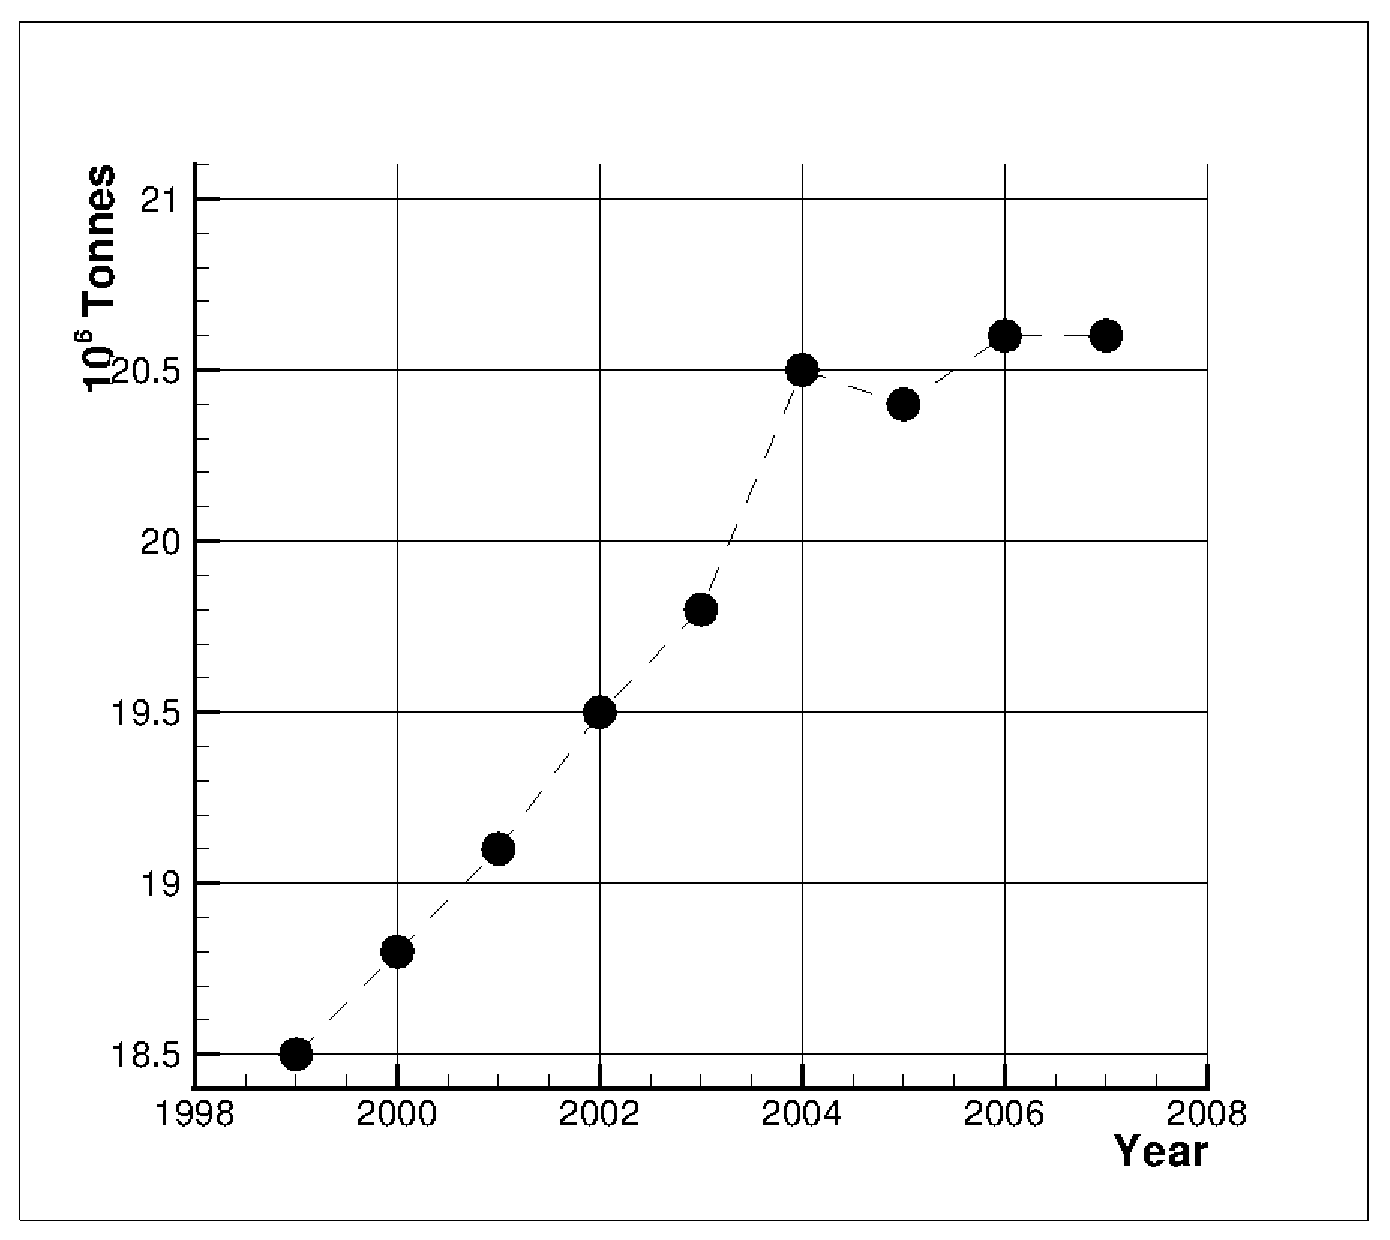
\includegraphics[scale=0.2]{atmosphereDynamic1}
			\caption{Динамика выбросов вредных веществ}\label{fig:emission}
		\end{figure}
	\end{minipage}
}
\subsection{Схема течения в циклоне}
\frame{\frametitle{Схема течения в циклоне}
	\begin{minipage}{0.69\linewidth}
		\centering
		\begin{itemize}
			\item Запылённый воздух входит в циклон через тангенциальный патрубок и, приобретая вращательное движение, опускается винтообразно вниз вдоль внутренних стенок цилиндра и конуса.
			\item Небольшая часть этого потока, в котором сконцентрированы пылевые частицы, движется в непосредственной близости от стенок циклона и поступает через пылеотводящее отверстие в пылесборный бункер, где происходит осаждение и накопление пылевых частиц.
			\item В центральной зоне циклона воздушный поток, освобождённый от пыли, поднимается винтообразно вверх и удаляется через выхлопную трубу наружу.		
		\end{itemize}
	\end{minipage}
	\hfill
	\begin{minipage}{0.3\linewidth}
		\centering
		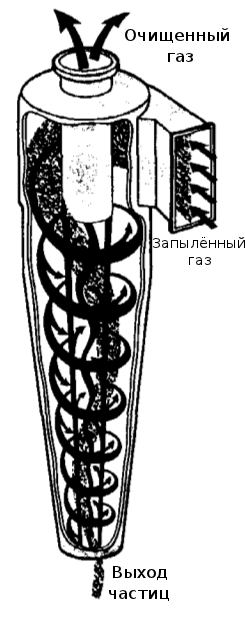
\includegraphics[scale=0.3]{flowScheme}	
	\end{minipage}
}
\subsection{Цели работы}
\frame{\frametitle{Цели работы}
	\begin{enumerate}
		\item Реализация $k-\omega-SST$ модели турбулентности с поправкой на кривизну линий тока при помощи открытой интегрируемой платформы для численного моделирования задач механики сплошных сред OpenFOAM.
		\item Реализация с использованием OpenFOAM солвера, имеющего в основе модель идеального газа и учитывающего при этом обратное влияние частиц на поток.
		\item Численное моделирование циклона с учётом обратного влияния частиц на поток и поправки на кривизну линий тока к генерации турбулентности.
	\end{enumerate}
}
\section*{Реализация поправки на кривизну линий тока}
\subsection{SST - модель с поправкой на кривизну}
\frame{\frametitle{Формулировка SST-модели с поправочным коэффициентом Шура-Спалларта}

Уравнение переноса $k$
	\begin{equation}
				\frac{\partial \rho k}{\partial t} + \frac{\partial \rho U_j k}{\partial x_j} = \tilde{P}_k f_{rot} - \beta^* \rho k \omega + \frac{\partial}{\partial x_j}(\Gamma_k \frac{\partial k}{\partial x_j}),
				\end{equation}
							
			Уравнение переноса $\omega$
				\begin{equation}
				\frac{\partial \rho \omega}{\partial t} + \frac{\partial U_j \omega}{\partial x_j} = \frac{\gamma}{\nu_t}P_kf_{rot} - \beta\rho\omega^2 + \frac{\partial}{\partial x_j}(\Gamma_{\omega}\frac{\partial \omega}{\partial x_j}) + (1-F_1)2\rho \sigma_{\omega_2}\frac{1}{\omega}\frac{\partial k}{\partial x_j}\frac{\partial \omega}{\partial x_j},
			\end{equation}

		
		Уравнения для поправочного коэффициента $f_{rot}$
\begin{equation}
				f_{r1}(r^*,\tilde{r}) = 2r^*\left( \frac{1+C_{r1}}{1+ r^*} \right)\left[ 1-C_{r3}\arctan{(C_{r2}\tilde{r})} \right] - C_{r1},
		\end{equation}
		\begin{equation}
				\tilde{r} = 2\Omega_{ik}S_{kj}\frac{DS_{ij}}{Dt}\frac{1}{\Omega D^3}, \quad D^2 = \max(S^2, 0.09 \omega^2),
		\end{equation}
		$$
				S^2 = 2 S_{ij}S_{ij}, \quad \Omega^2 = 2 \Omega_{ij} \Omega_{ij}, \quad r^* = S/\Omega
		$$
		$$
				C_{r1} = 1, \quad C_{r2} = 2, \quad C_{r3} = 1, \quad f_{rot} = \max[\min(f_{r1},1.25),0]
		$$
}
\subsection{Верификация реализованной поправки}
\frame{\frametitle{Постановка задачи}
	\begin{minipage}{0.59\linewidth}
		\vspace{-10em}
		\begin{figure}[h]
		\centering
		\includegraphics[scale=0.3]{UDuct}
		\caption{Геометрия канала}
		\end{figure}
	\end{minipage}	
	\begin{minipage}{0.4\linewidth}
		\begin{figure}[h]
			\centering
			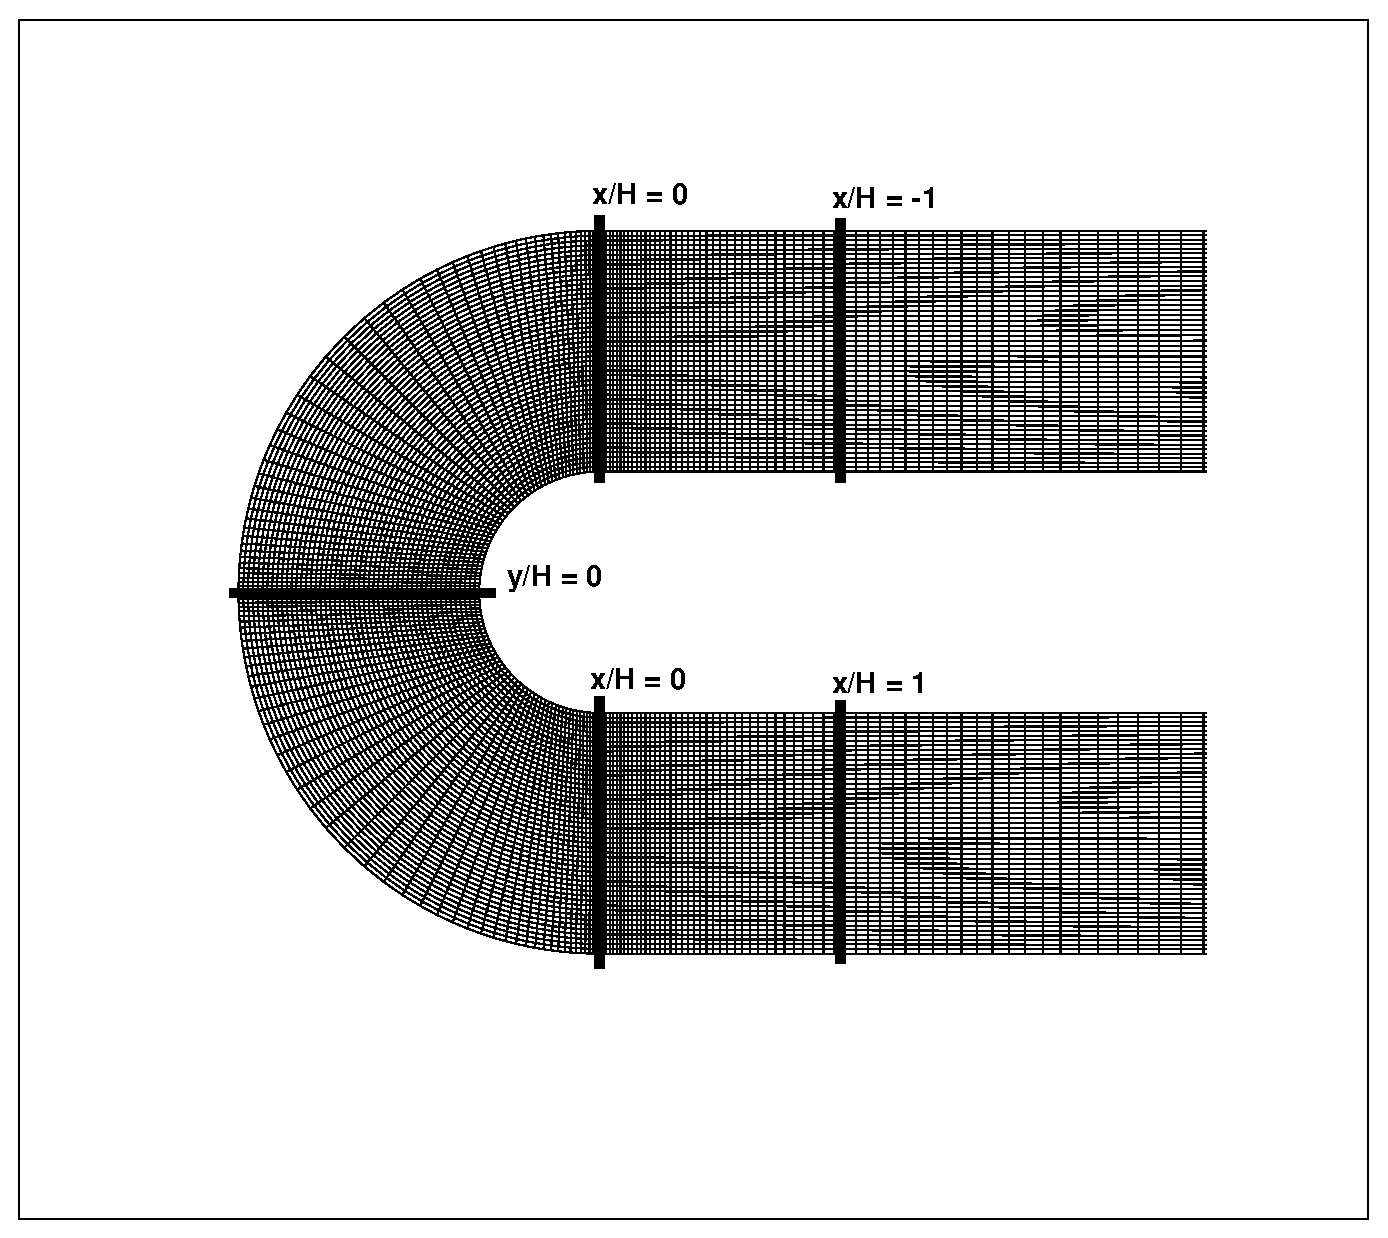
\includegraphics[scale=0.2]{sampleLinesAndMesh}
			\caption{Сетка расчётной области на участке поворота}
		\end{figure}
	\end{minipage}
	\begin{minipage}{0.5\linewidth}
		\vspace{-9em}
		\centering
		\begin{table}
		
			\begin{tabular}{r l}
			\hline \\
				\label{tableUDuct}
				Высота, & $H=3.81cm$ \\
				Длина канала, & $L = 10H$ \\
				Внутренний радиус, & $R_i = 1.91cm$ \\
				Внешний радиус, & $R_o = 5.72cm$ \\
				Ср. скорость на входе, & $U_{in} = 30.1 m/s$ \\
				Температура на входе, & $T_{in} = 264 K$ \\
			\end{tabular}
			\end{table}
	\end{minipage}
}
\frame{\frametitle{Методические исследования}
		\begin{minipage}[t]{0.49\linewidth}
		\begin{figure}[t]
		\centering
		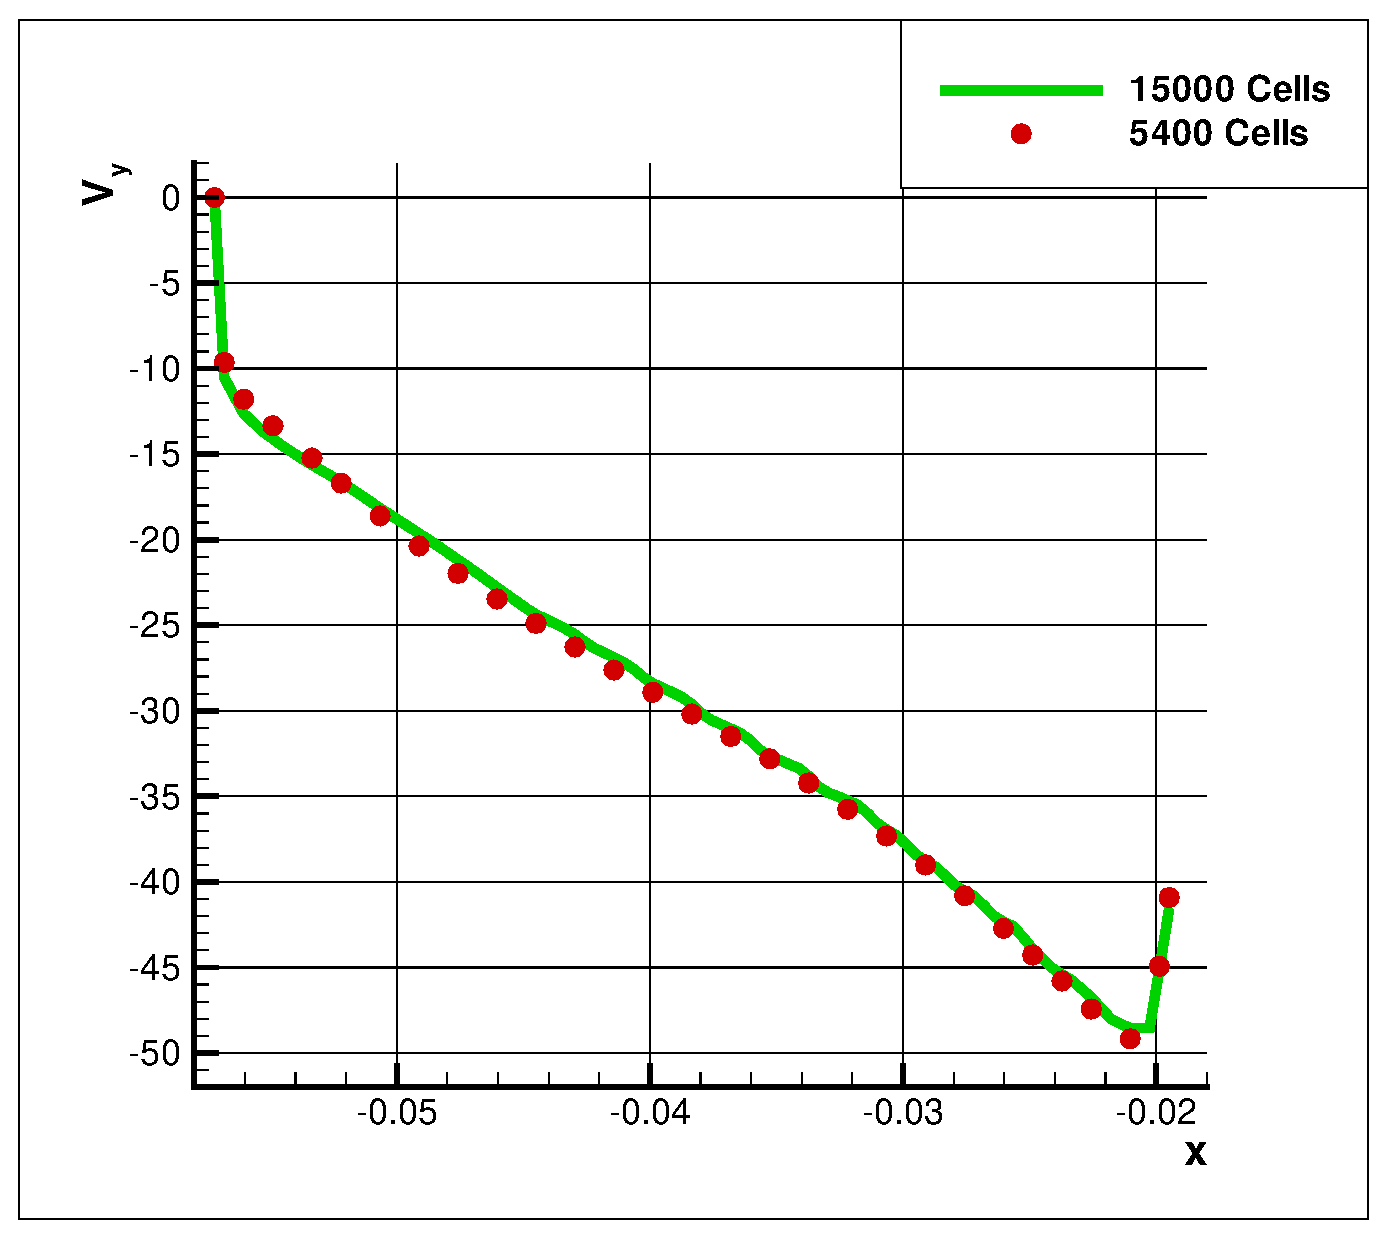
\includegraphics[scale=0.25]{uDuctMeshIndependence2Color}
		\caption{Сравнение профилей $V_y$ в сечении $y=0$ для разных сеток}
		\end{figure}
	\end{minipage}
	\begin{minipage}[t]{0.49\linewidth}
		\begin{figure}[t]
		\centering
		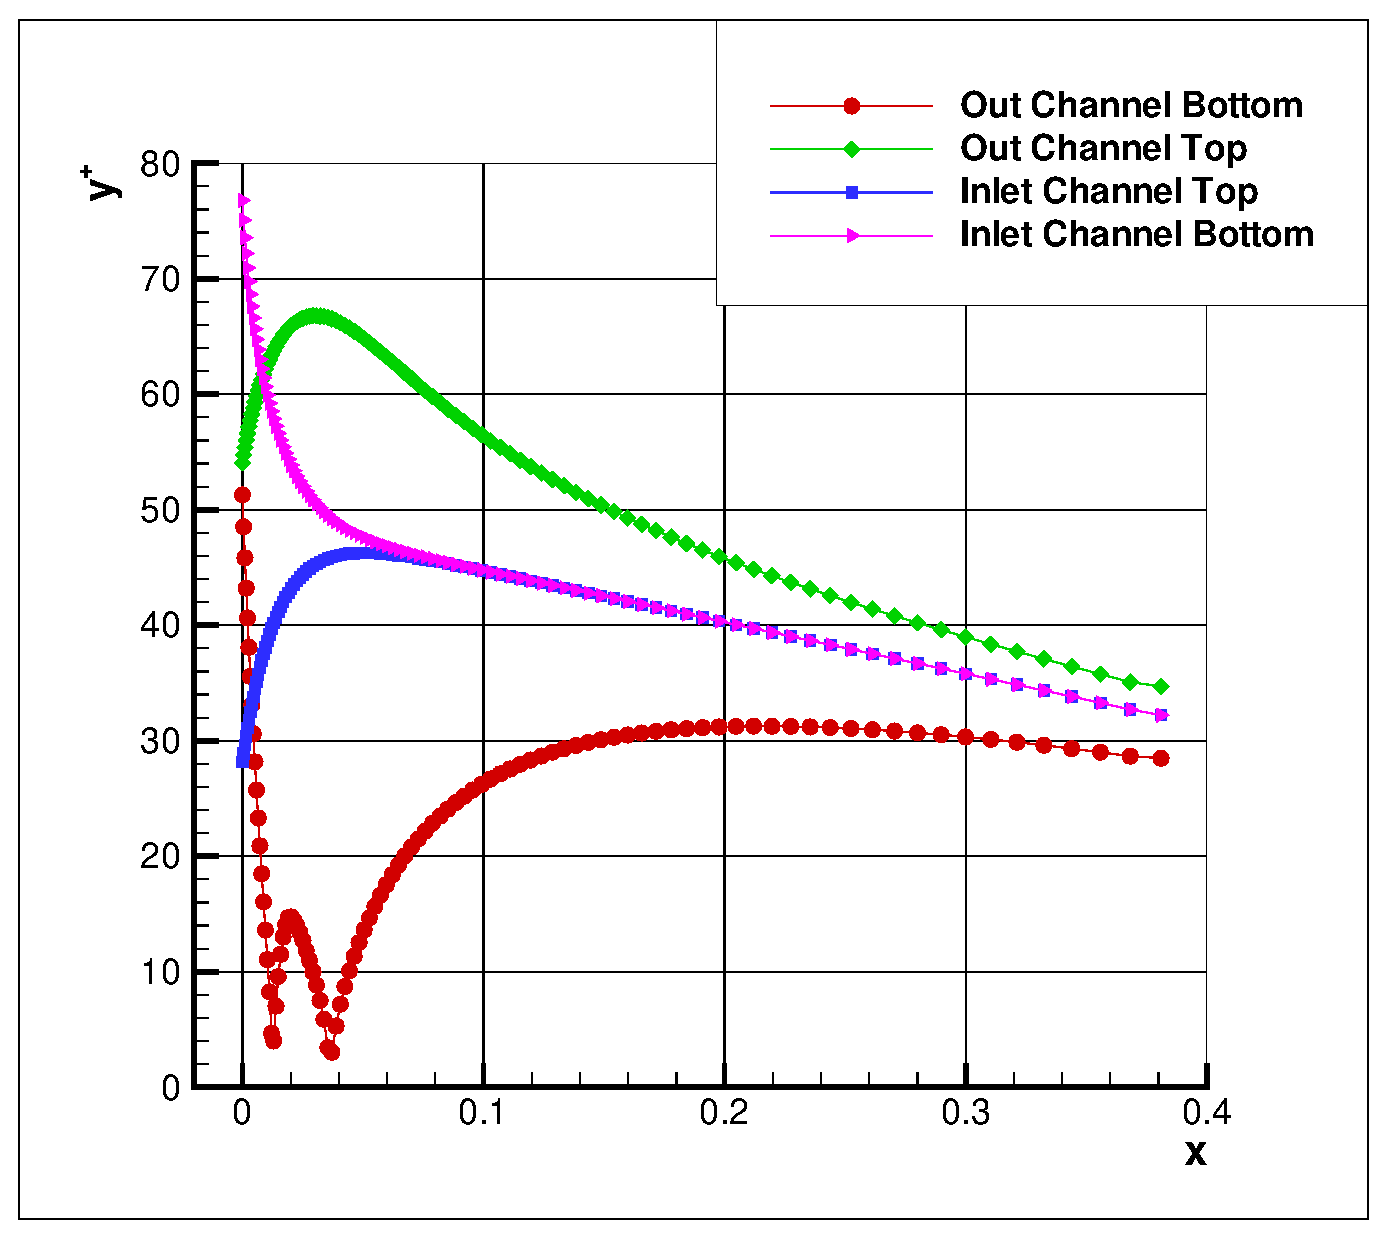
\includegraphics[scale=0.25]{uDuctyplusColor}
		\caption{Величина $y^{+}$ первой пристенной ячейки на внешней и внутренней стенках}
		\end{figure}
	\end{minipage}
}
\frame{\frametitle{Сравнение с экспериментами Монсона и моделированием в Fluent}
	\vspace{-1.1em}
	\begin{minipage}[t]{0.49\linewidth}
		\begin{figure}[t]
			\centering
		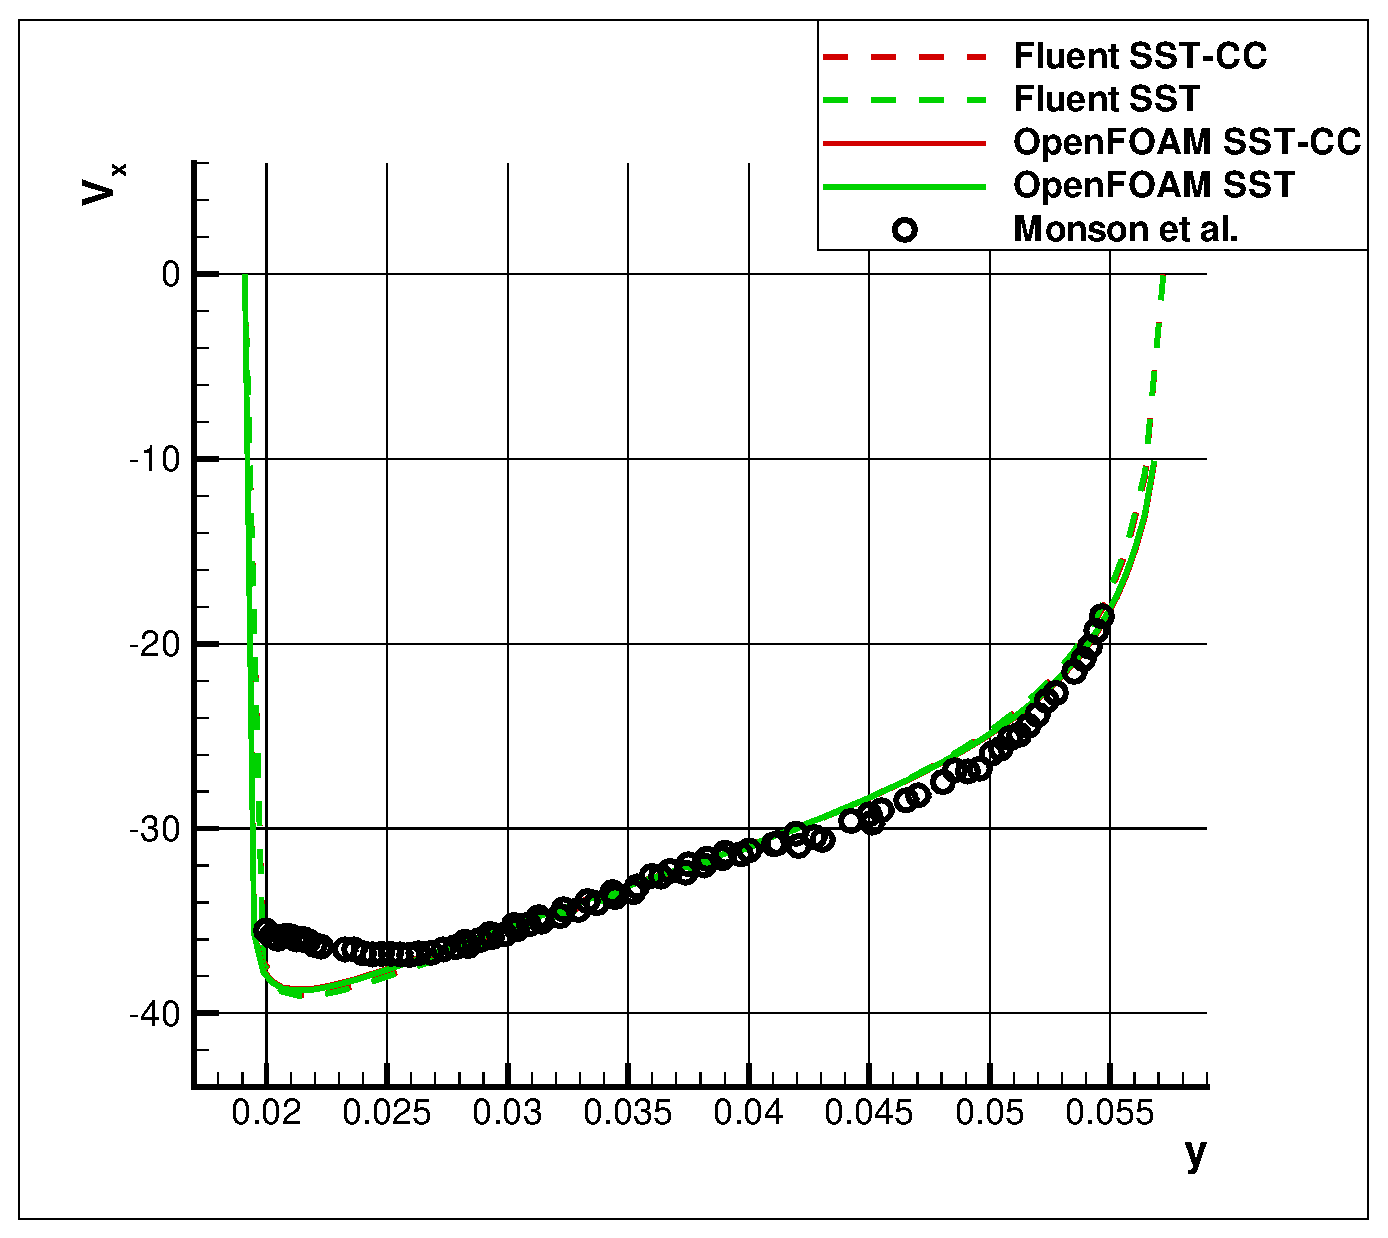
\includegraphics[scale=0.15]{xh0up}
		\caption{Профиль $V_x$ в сечении $x/H=0$ (верх)}
		\end{figure}
	\end{minipage}
	\begin{minipage}[t]{0.49\linewidth}
		\begin{figure}[t]
			\centering
		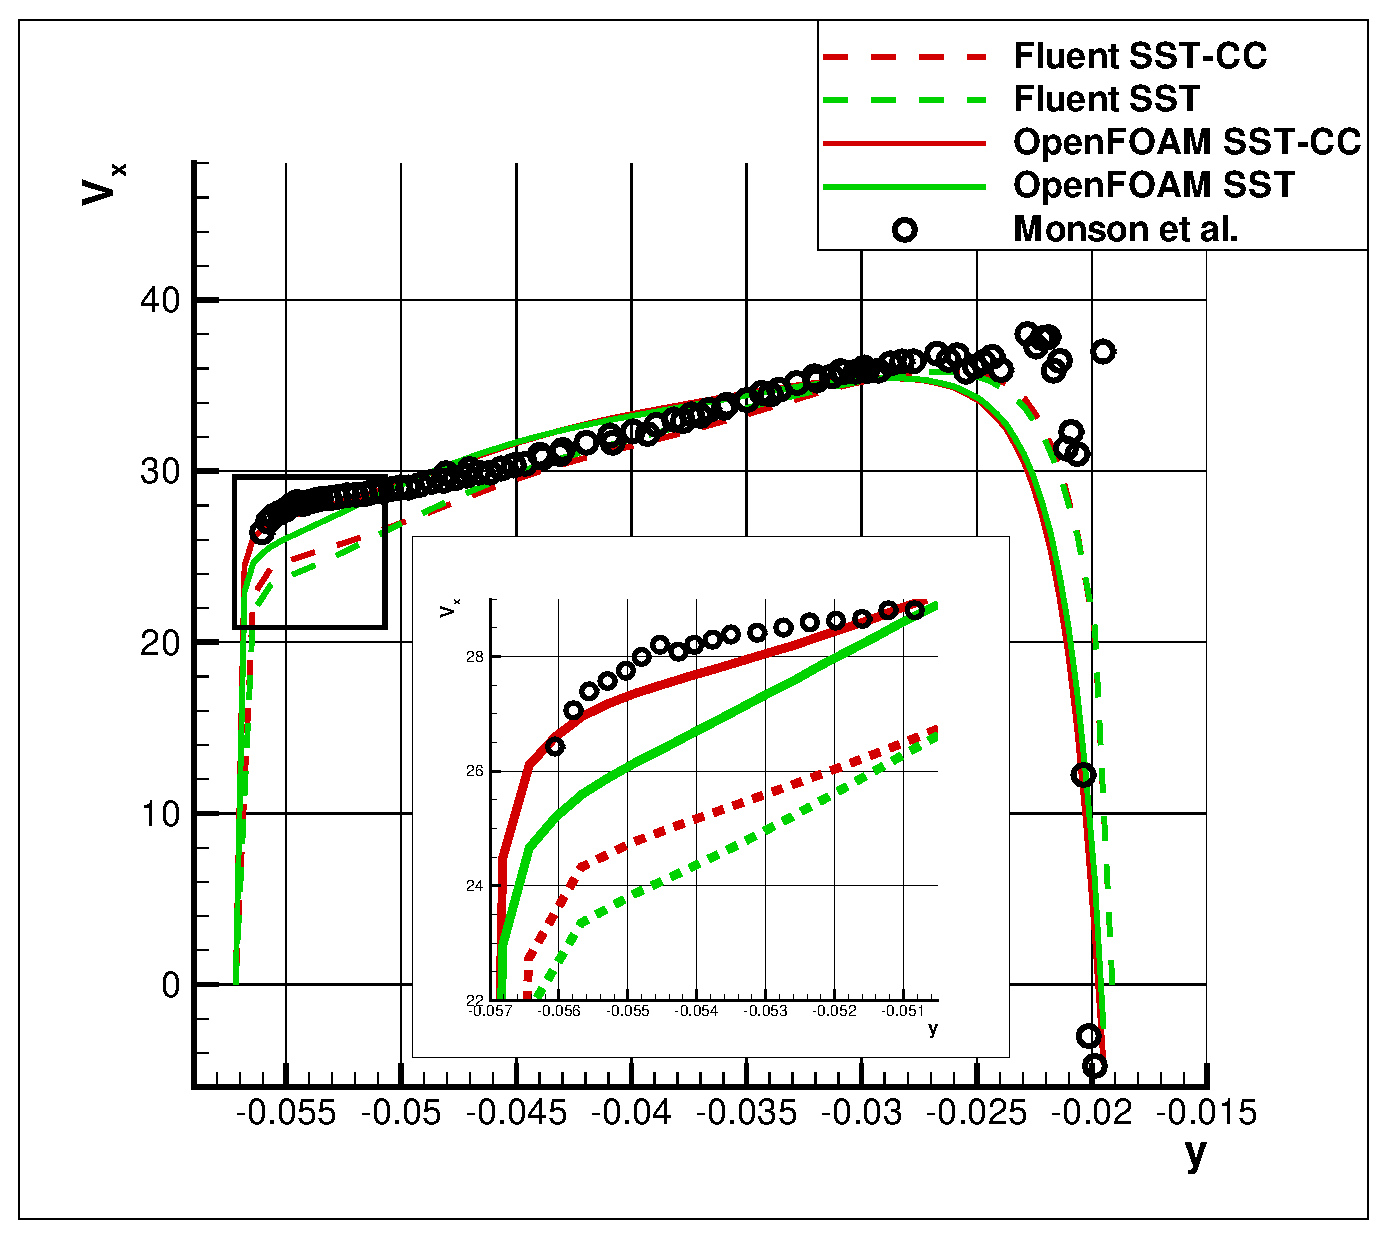
\includegraphics[scale=0.15]{xh0down}
		\caption{Профиль $V_x$ в сечении $x/H=0$ (низ)}
		\end{figure}
	\end{minipage}
	\begin{minipage}[t]{0.49\linewidth}
		\vspace{-0.5em}
		\begin{figure}[t]
			\centering
		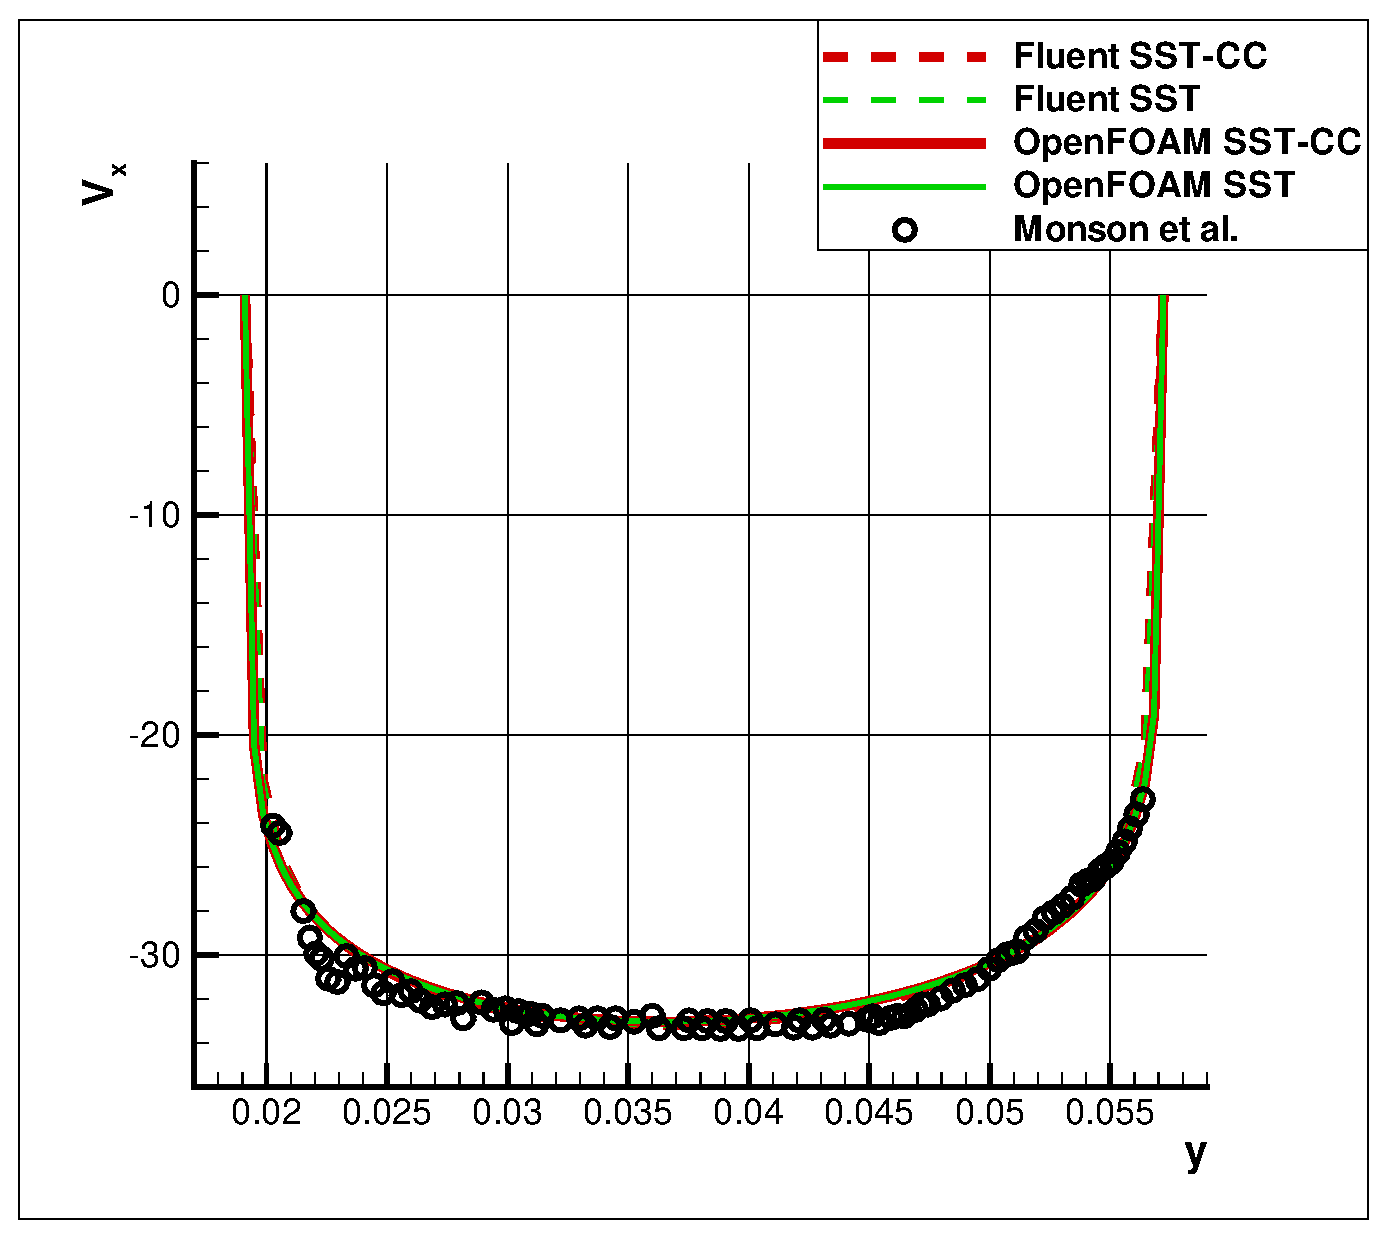
\includegraphics[scale=0.15]{xh1up}
		\caption{Профиль $V_x$ в сечении $x/H=-1$}
		\end{figure}
	\end{minipage}
	\begin{minipage}[t]{0.49\linewidth}
		\vspace{-0.5em}
		\begin{figure}[t]
			\centering
		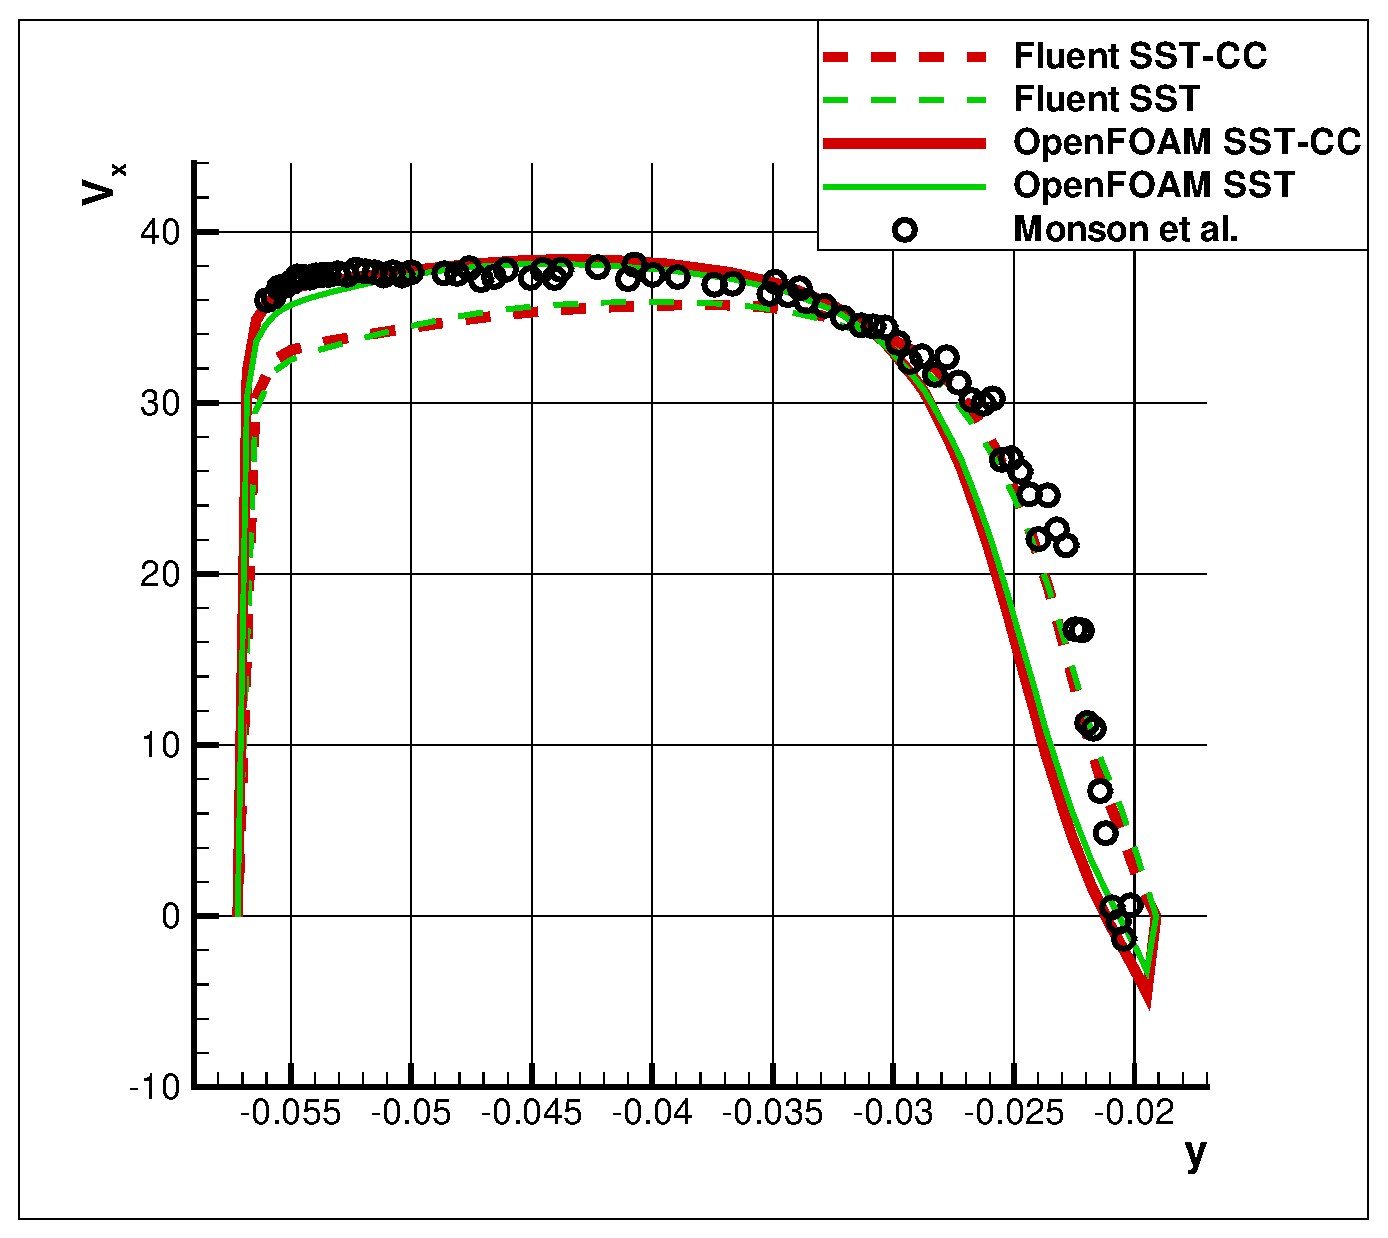
\includegraphics[scale=0.15]{xh1down}
		\caption{Профиль $V_x$ в сечении $x/H=1$}
		\end{figure}
	\end{minipage}
}
\section*{Численное моделирование циклона}
\subsection{Решение без дисперсных включений}
\frame{\frametitle{Геометрия фильтра}
	\small{
		\hspace{0.02\textwidth}
		\begin{minipage}[t]{0.5\linewidth}
			\vspace{0.2\textwidth}
			\begin{table}[h]
			\begin{tabular}{c c}
				\label{geometrytable}
				Диаметр цилиндра, $D$ & $0.205m$ \\
				Диаметр выходной трубы, $D_e$ & $0.5D$ \\
				Высота входного канала, $a$ & $0.5D$ \\
				Ширина входного канала, $b$ & $0.2D$ \\
				Длина выходной трубы, $h_e$ & $0.75D$ \\
				Полная высота фильтра, $H$ & $4.0D$ \\
				Высота цилиндра, $h$ & $1.5D$ \\
				Диаметр нижнего сечения фильтра, $B$ & $0.36D$ \\
				Диаметр пылесборника, $D_d$ & $0.75D$ \\
			\end{tabular}
		\end{table}
	\end{minipage}
	\hfill
	\begin{minipage}[t]{0.45\linewidth}
		\centering
		\vspace{-1.5ex}
		\begin{figure}
			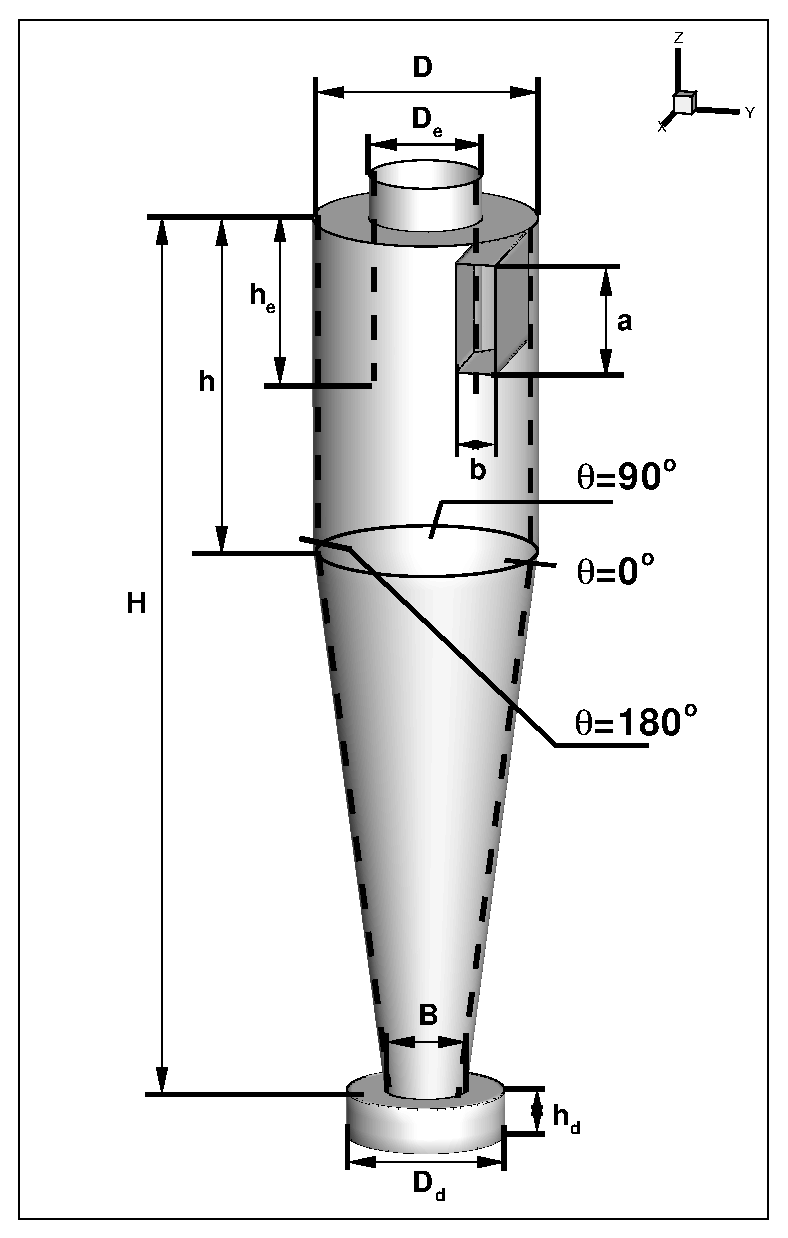
\includegraphics[scale=0.3]{cycloneGeometryTeta}
			\caption{Схема фильтра}\label{fig:geometry}
		\end{figure}
	\end{minipage}
	}
}
\frame{
	\frametitle{Постановка задачи}\small{
	\begin{minipage}[t]{0.6\linewidth}
		\vspace{0.2\textwidth}
		\begin{table}
			\begin{tabular}{c}
				Средняя скорость на входе, $U_{in}=$ $5, 10, 15$ и $20m/s$\\
				Температура воздуха на входе, $T_{in}=$  $300 K$ \\
				Тепловой поток на стенках, $q_w=$  $0$ \\
				Давление в выходном сечении, $p_{out}=$  $1 atm$ \\
				Скорость частиц на входе, $U_{p,in}=$ $U_{in}$ \\
				Температура частиц на входе, $T_{p,in}=$ $T_{in}$\\
				Диаметры частиц, $d_p=$ $\sim 10^{-5}, 10^{-6}, 10^{-7} m$
			\end{tabular}
		\end{table}
	\end{minipage}
%	\hspace{\textwidth}
	\begin{minipage}[t]{0.39\linewidth}
		\begin{figure}[t]
			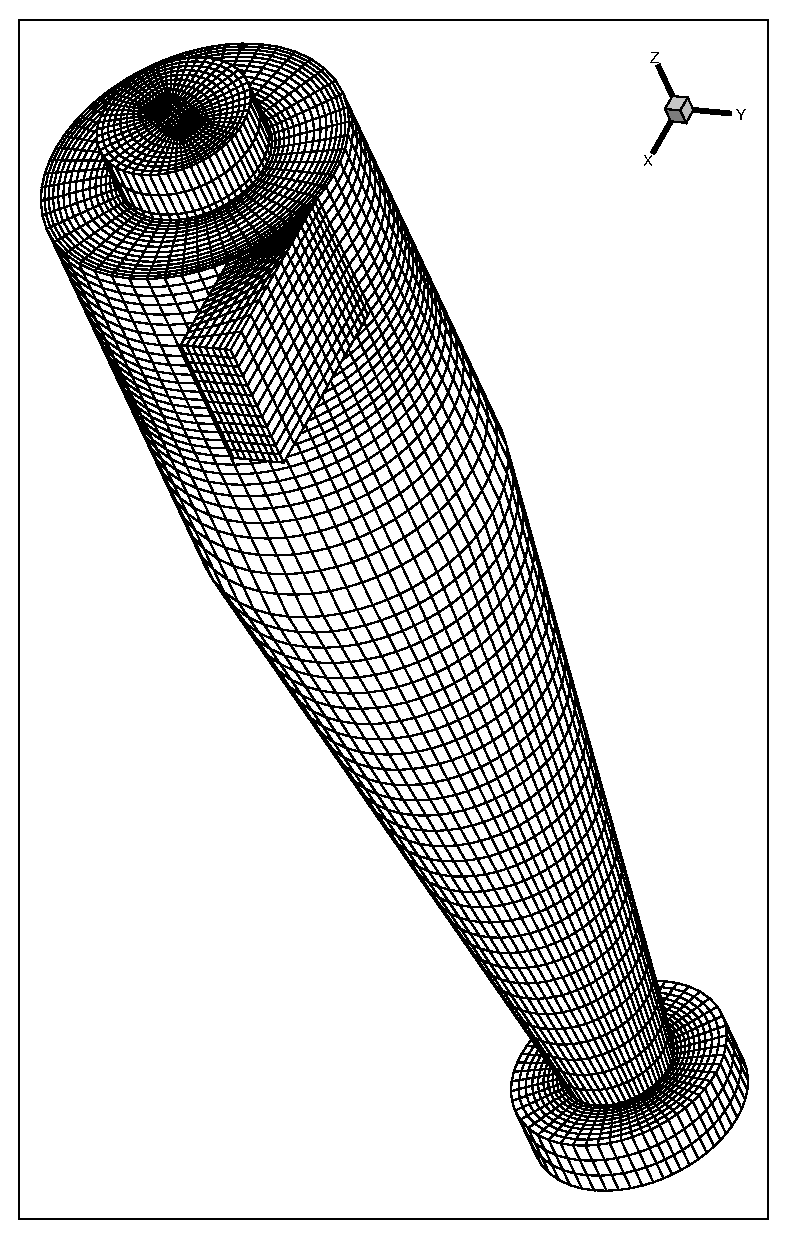
\includegraphics[scale=0.3]{meshCyclone}
			\caption{Расчётная сетка}
		\end{figure}
	\end{minipage}
	}
}
\frame{\frametitle{Методические исследования}
	\begin{minipage}[t]{0.49\linewidth}
		\begin{figure}[t]
		\centering
		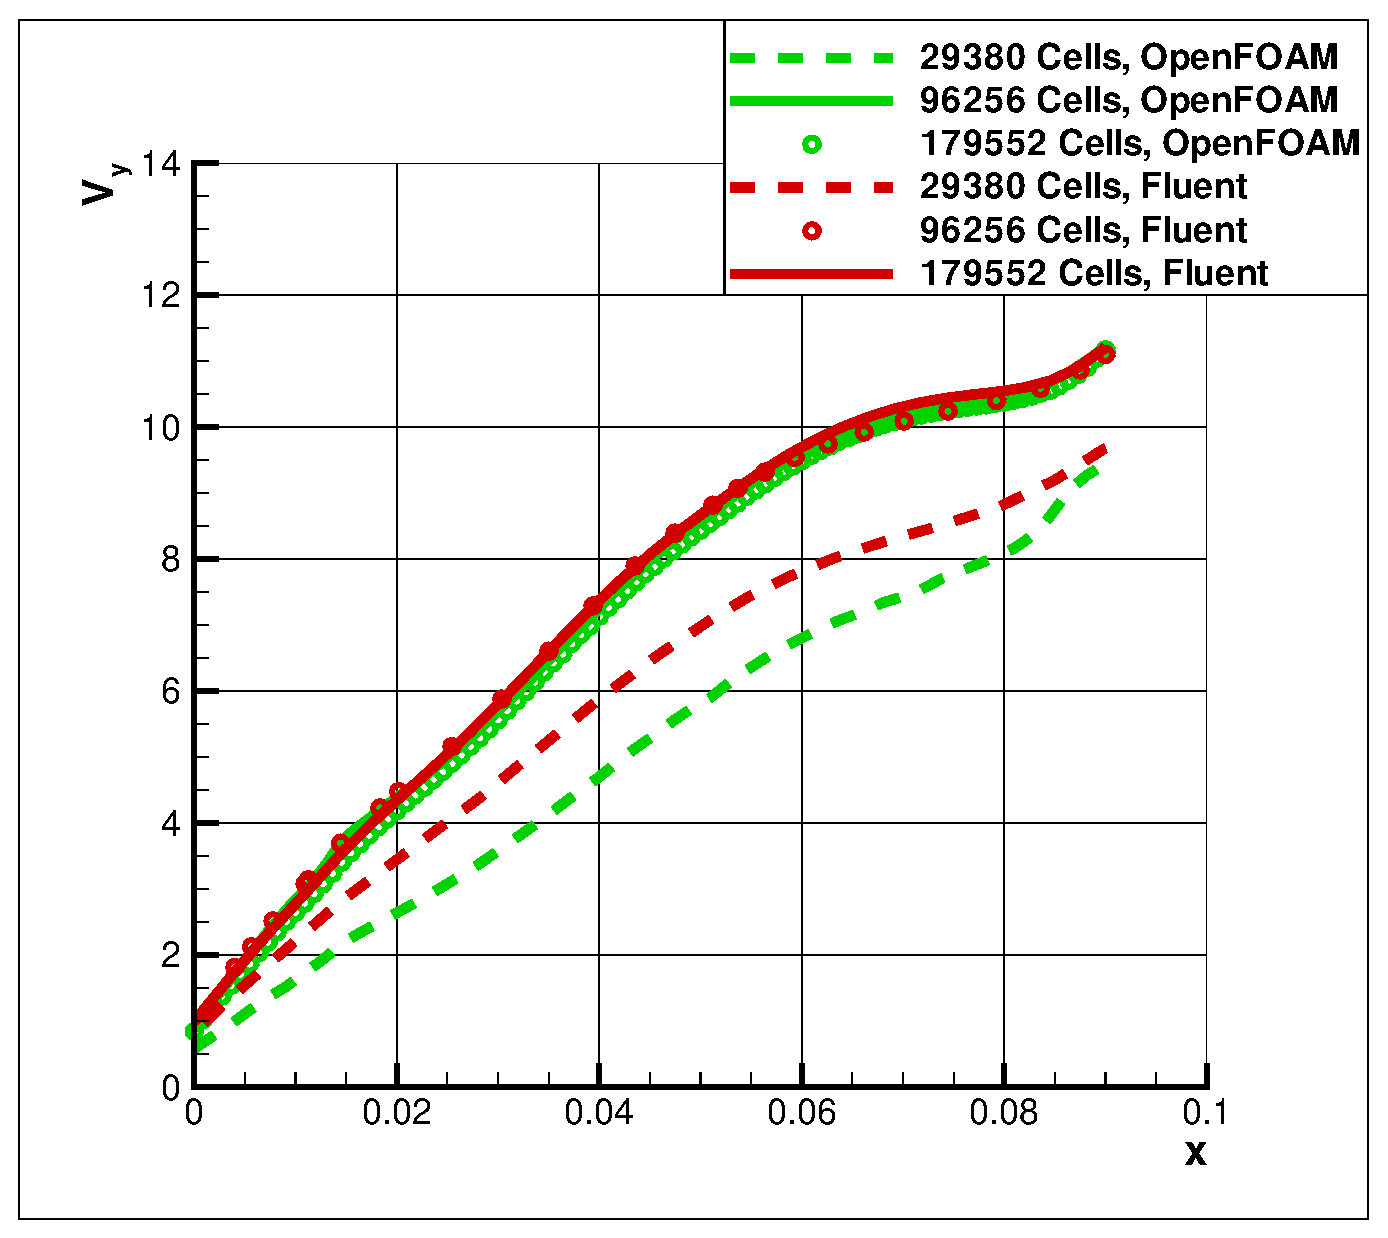
\includegraphics[scale=0.25]{cycloneMeshIndependence1Color}
		\caption{Профили $V_y$ вдоль прямой $z=-0.3m$, $y=0$}
		\end{figure}
	\end{minipage}
	\begin{minipage}[t]{0.49\linewidth}
		\begin{figure}[t]
		\centering
		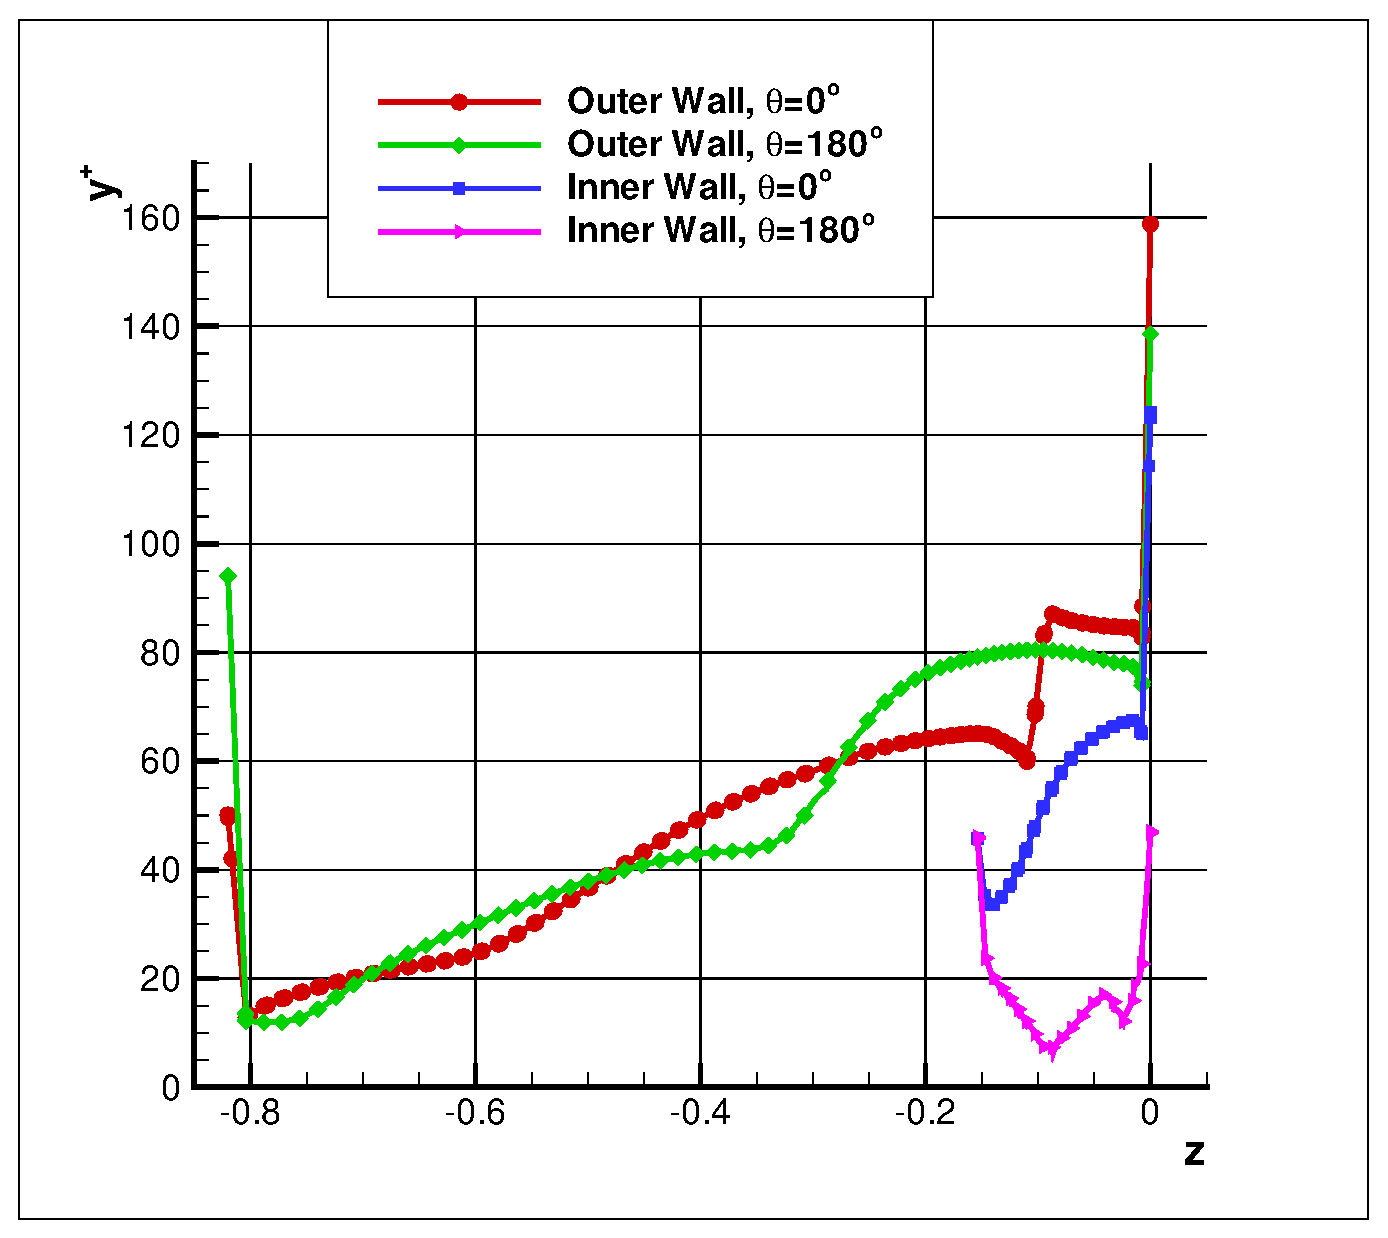
\includegraphics[scale=0.25]{yplusCycloneColor}
	\caption{Величина $y^{+}$ первой пристенной ячейки на внешней и внутренней стенках циклона}
		\end{figure}
	\end{minipage}
}
\frame{\frametitle{Влияние поправки на течение в циклоне}
	\vspace{-1.1em}
	\begin{minipage}[t]{0.49\linewidth}
		\begin{figure}[t]
			\centering
		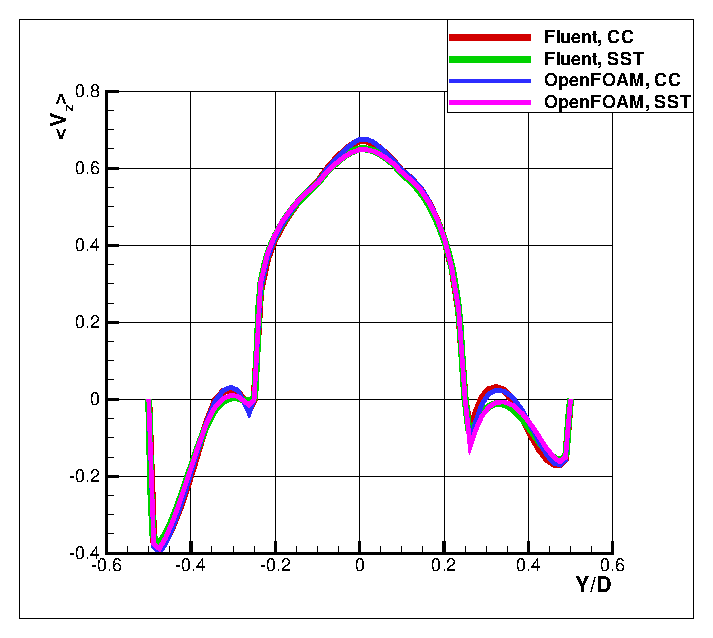
\includegraphics[scale=0.3]{axialCyclone}
\caption{Профили $V_{z}/U_{in}$ вдоль прямой $Z/D=-0.75, x=0$}
		\end{figure}
	\end{minipage}
	\begin{minipage}[t]{0.49\linewidth}
		\begin{figure}[t]
			\centering
		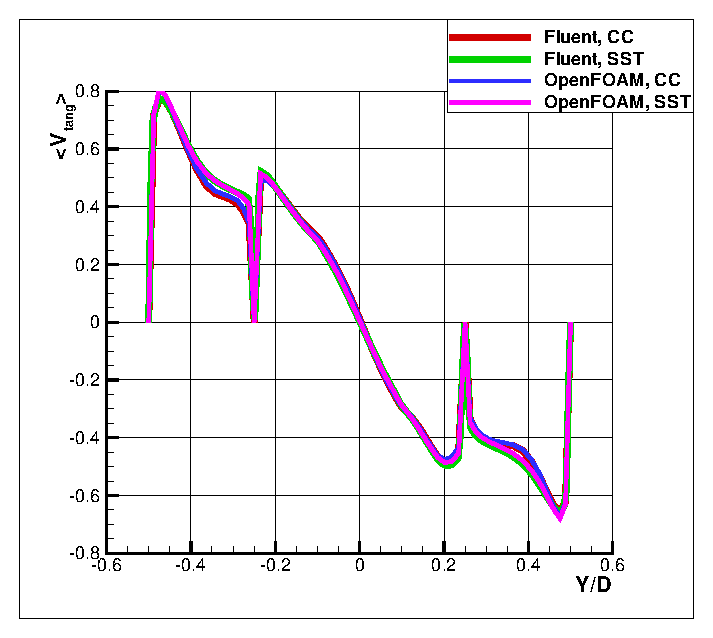
\includegraphics[scale=0.3]{tangentialCyclone}
		\caption{Профили $V_{tg}/U_{in}$ вдоль прямой $Z/D=-0.75, x=0$}
		\end{figure}
	\end{minipage}
	\begin{minipage}[t]{0.49\linewidth}
		\vspace{-0.5em}
		\begin{figure}[t]
			\centering
		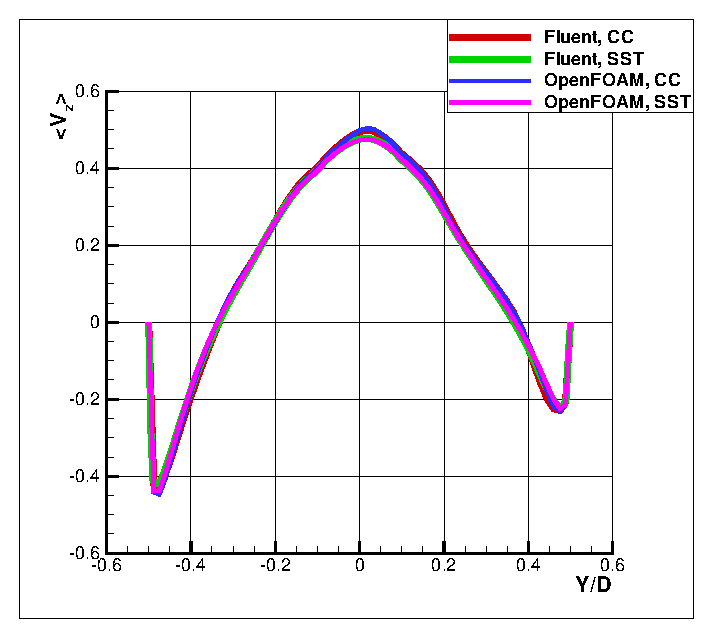
\includegraphics[scale=0.3]{axialCyclone2}
		\caption{Профили $V_{z}/U_{in}$ вдоль прямой $Z/D=-1, x=0$}
		\end{figure}
	\end{minipage}
	\begin{minipage}[t]{0.49\linewidth}
		\vspace{-0.5em}
		\begin{figure}[t]
			\centering
		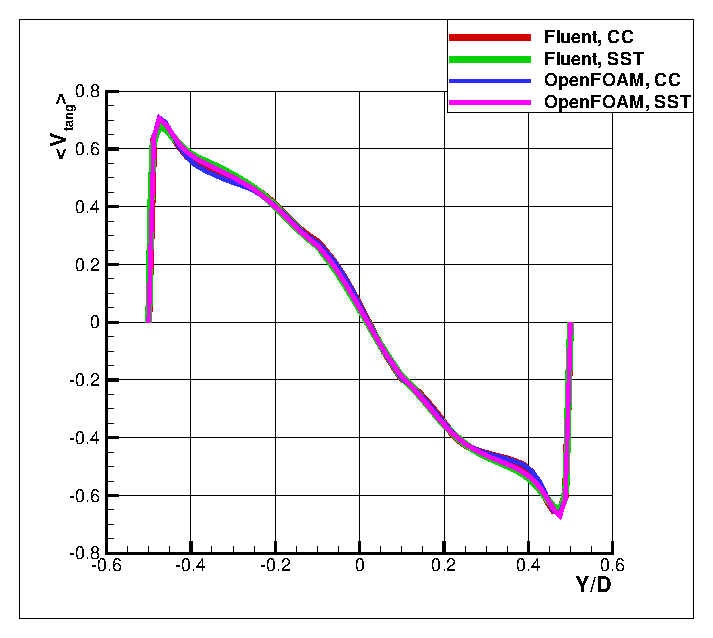
\includegraphics[scale=0.3]{tangentialCyclone2}
		\caption{Профили $V_{tg}/U_{in}$ вдоль прямой $Z/D=-1, x=0$}
		\end{figure}
	\end{minipage}
}
\subsection{Расчёт траекторий частиц}
\frame{\frametitle{Модель частиц в OpenFOAM}
	\begin{minipage}[t]{0.6\linewidth}
		Уравнение движения частицы в OpenFOAM:
		\small{
			\begin{equation}
				\label{particle}
					m_p \frac{d \vec{V}_p}{dt} = \frac{1}{2}\rho |\vec{V}-\vec{V}_p|(\vec{V}-\vec{V}_p)\frac{d_p^2 \pi}{4}C_D + m_p \vec{g} + \vec{F}_{\nabla{p}}
			\end{equation}
		}
		\small{
			\begin{table}[t]
				\begin{tabular}{r l}
					$m_p$ & -- масса частицы\\
					$\vec{V}_p$ & -- скорость частицы\\
					$\vec{V}$ & -- скорость жидкости\\
					$C_D$ & -- коэффициент сопротивления\\
					$\rho$ & -- плотность жидкости \\
					$\vec{F}_{\nabla{p}}$ & -- сила, обусловленная действием градиента давления
				\end{tabular}
			\end{table}
		}
		\begin{itemize}
			\item Cell-to-face-to-cell tracking для траекторий частиц.
			\item Если необходимы более детальные траектории используются дополнительные циклы решения внутри ячеек.
			\item Для решения уравнения (\ref{particle}) используется встроенный в OpenFOAM ODE солвер.
		\end{itemize}
	\end{minipage}
	\begin{minipage}[t]{0.3\linewidth}
		\vspace{0.3\textwidth}
		\begin{figure}
			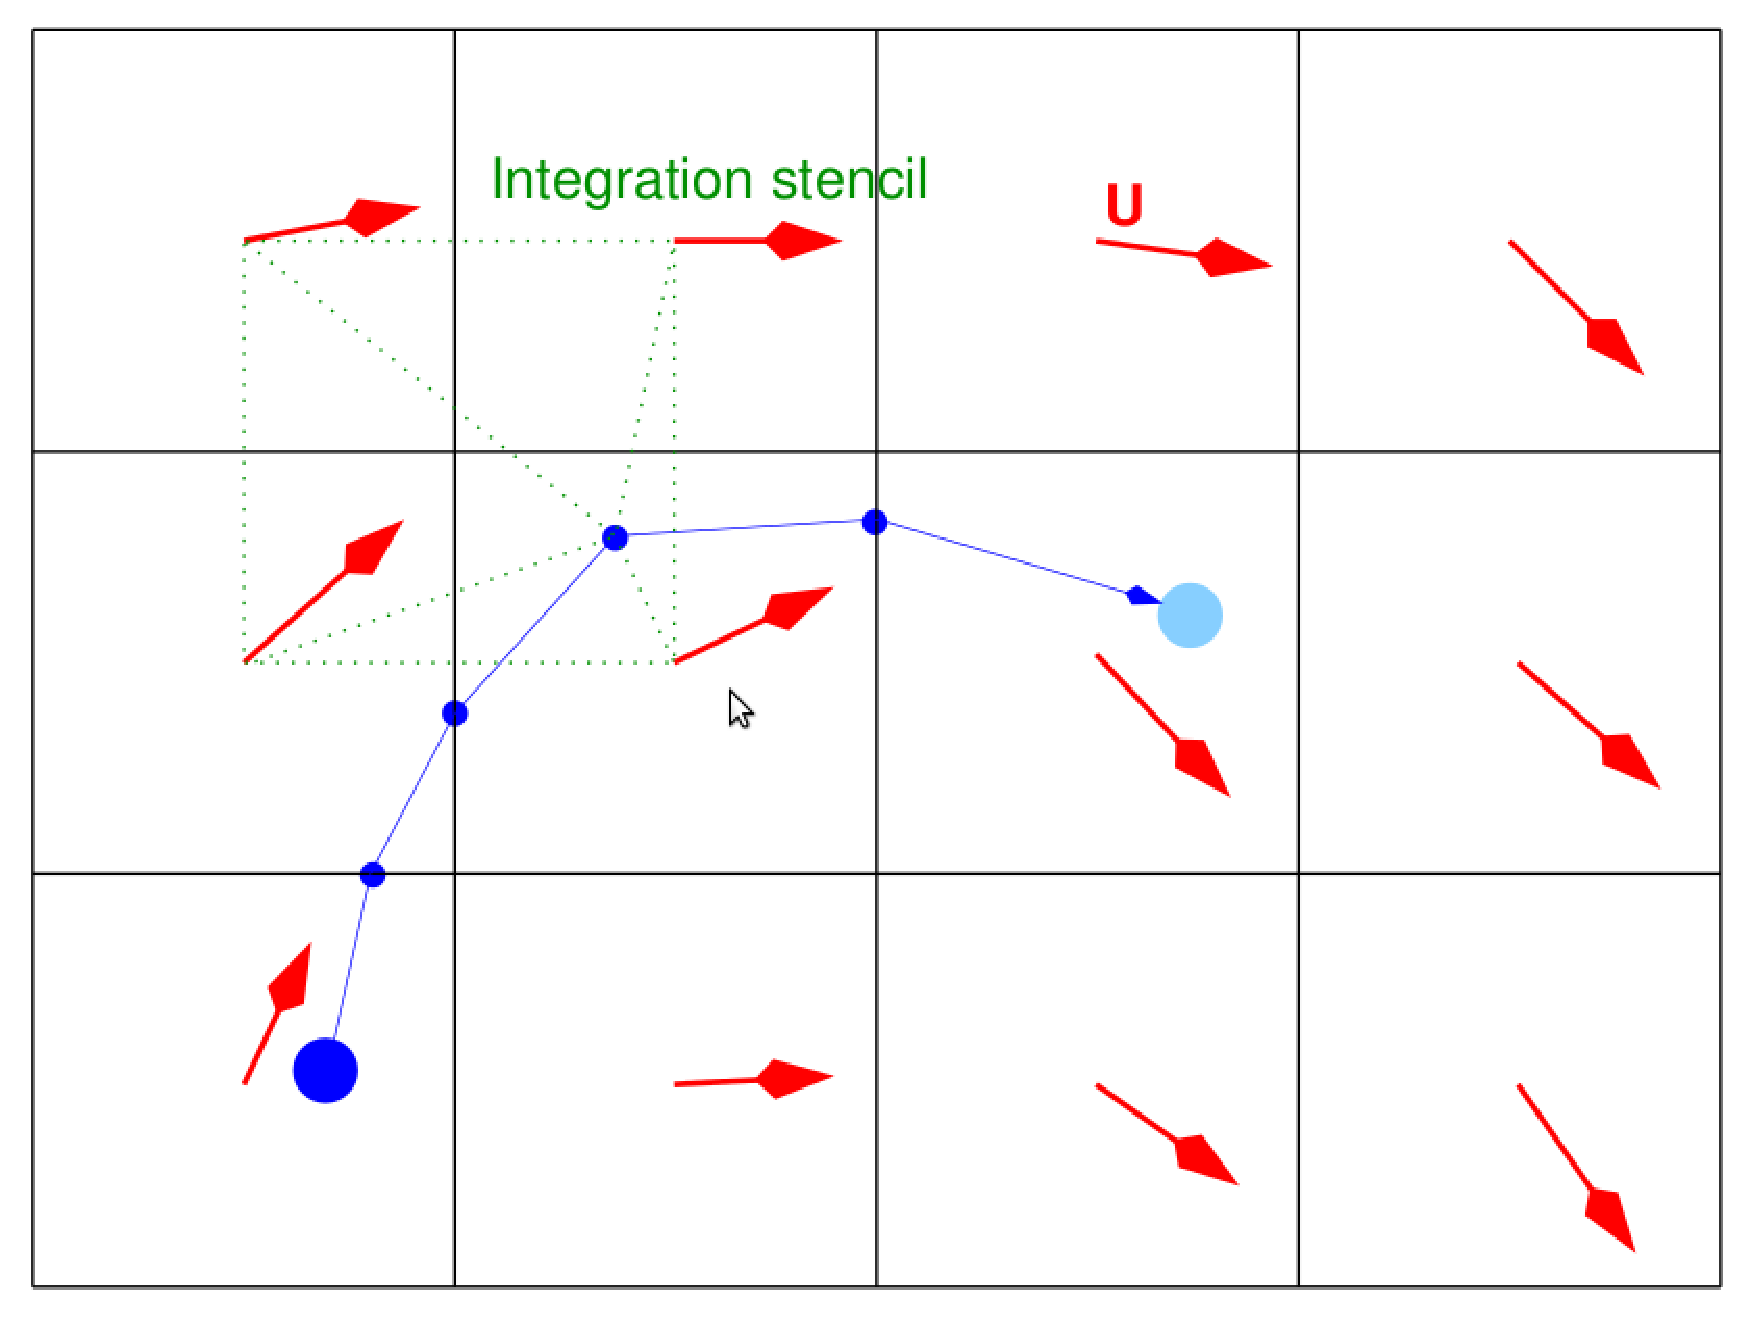
\includegraphics[scale=0.1]{particleJasak}
			\caption{Схема движения частиц}
		\end{figure}
	\end{minipage}
}
\frame{\frametitle{Развитие течения дисперсных включений во времени}
\begin{center}
	\begin{figure}[t]
 	\centering
	\begin{minipage}{0.2\linewidth}
	\centering
		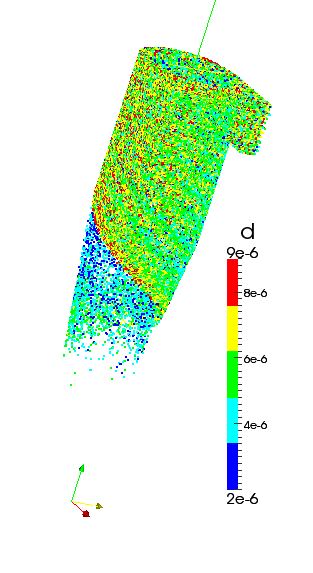
\includegraphics[scale=0.12]{t1}\\
		\text{t=0.1s}
	\end{minipage}
	\hspace{-1em}
	\begin{minipage}{0.2\linewidth}
	\centering
		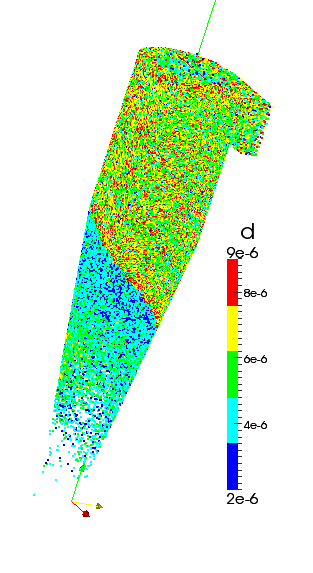
\includegraphics[scale=0.12]{t2}\\
		\text{t=0.2s}
	\end{minipage}
		\hspace{-1em}
	\begin{minipage}{0.2\linewidth}
	\centering
		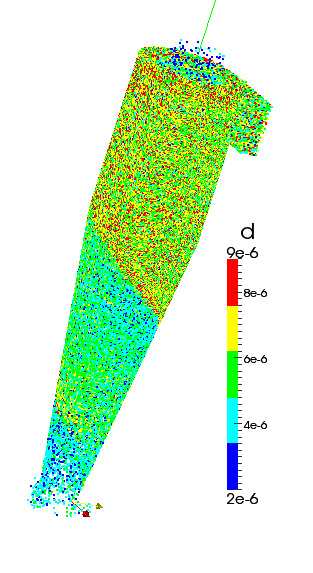
\includegraphics[scale=0.12]{t3}\\
		\text{t=0.3s}
	\end{minipage}
		\hspace{-1em}
	\begin{minipage}{0.2\linewidth}
	\centering
		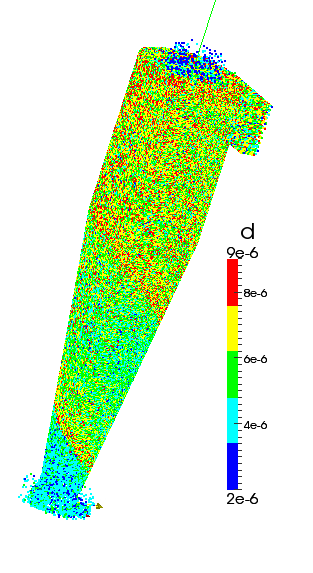
\includegraphics[scale=0.12]{t4}\\
		\text{t=0.4s}
	\end{minipage}
		\hspace{-1em}
	\begin{minipage}{0.2\linewidth}
	\centering
		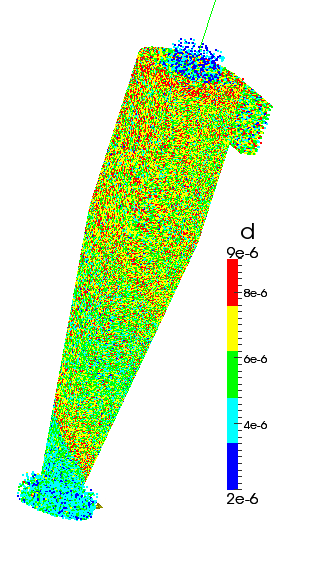
\includegraphics[scale=0.12]{t5}\\
		\text{t=0.5s}
	\end{minipage}
		\hspace{-1em}
	\begin{minipage}{0.2\linewidth}
	\centering
		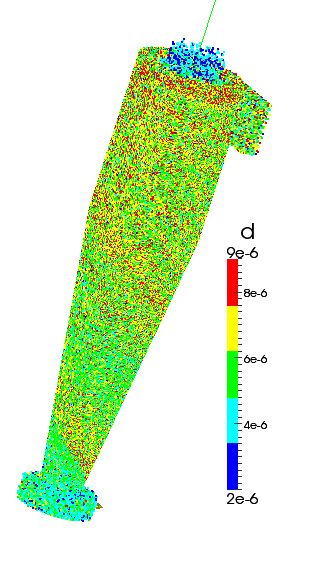
\includegraphics[scale=0.12]{t6}\\
		\text{t=0.6s}
	\end{minipage}
		\hspace{-1em}
	\begin{minipage}{0.2\linewidth}
	\centering
		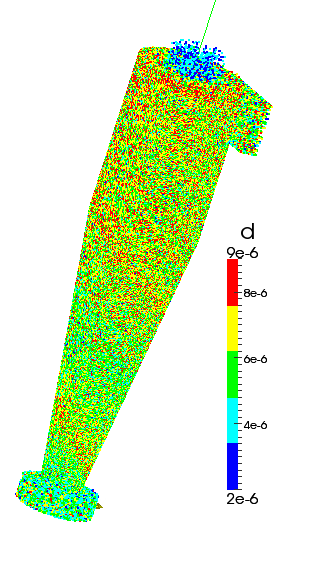
\includegraphics[scale=0.12]{t7}\\
		\text{t=0.7s}
	\end{minipage}
		\hspace{-1em}
	\begin{minipage}{0.2\linewidth}
	\centering
		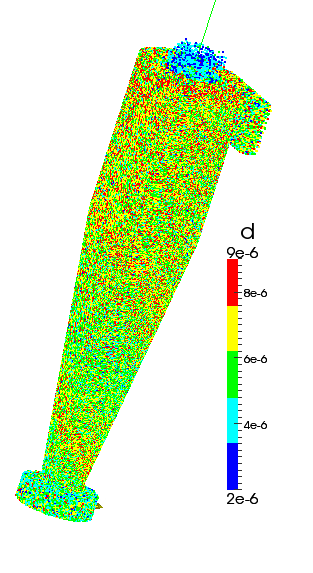
\includegraphics[scale=0.12]{t8}\\
		\text{t=0.8s}
	\end{minipage}
		\hspace{-1em}
	\begin{minipage}{0.2\linewidth}
	\centering
		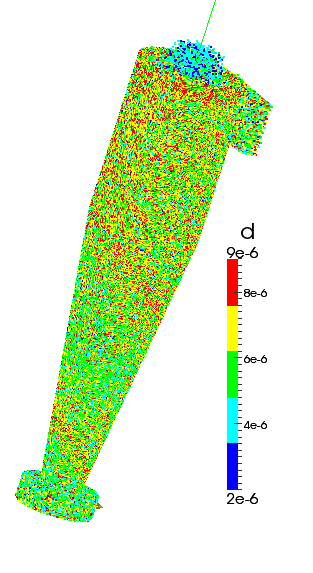
\includegraphics[scale=0.12]{t9}\\
		\text{t=0.9s}
	\end{minipage}
		\hspace{-1em}
	\begin{minipage}{0.2\linewidth}
	\centering
		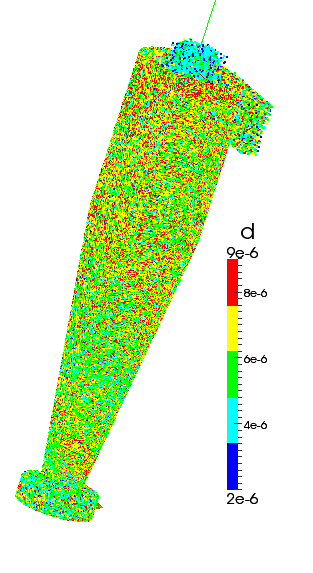
\includegraphics[scale=0.12]{t10}\\
		\text{t=1s}
	\end{minipage}
	\caption{Раcпределение дисперсных включений по диаметрам частиц для $U_{in} = 20m/s$, $d_p \sim 10^{-6}$}
\end{figure}
\end{Huge}
}
\frame{\frametitle{Распределение частиц для разных скоростей и диаметров}
	\begin{figure}[h]
	\centering
	\begin{minipage}{0.475\linewidth}
	\centering
		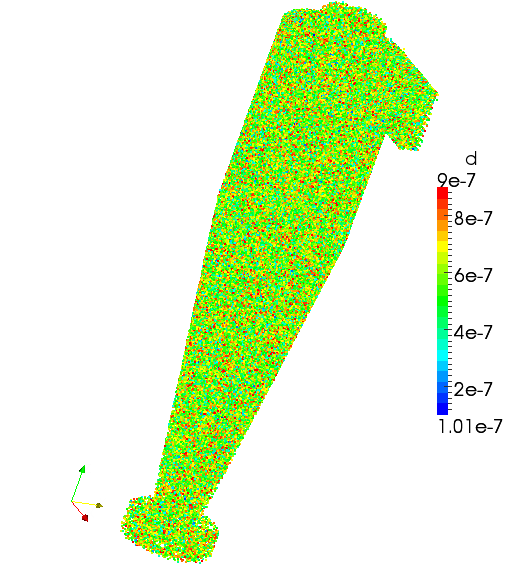
\includegraphics[scale=0.12]{parcelsCyclone1}\\
		\text{$d \sim 10^{-7}$, $U_{in} = 20m/s$}
	\end{minipage}
	\hspace{0.5em}
	\begin{minipage}{0.475\linewidth}
	\centering
		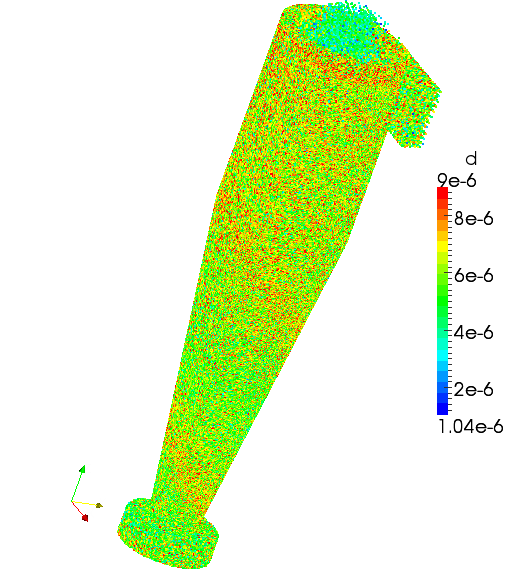
\includegraphics[scale=0.12]{parcelsCyclone2}\\
		\text{$d \sim 10^{-6}$, $U_{in} = 20m/s$}
	\end{minipage}
	\begin{minipage}{0.475\linewidth}
	\centering
		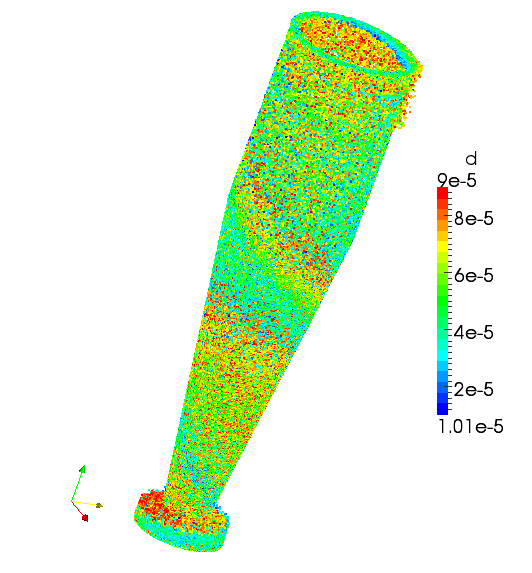
\includegraphics[scale=0.12]{parcelsCyclone3}\\
		\text{$d \sim 10^{-5}$, $U_{in} = 20m/s$}
	\end{minipage}
	\hspace{0.5em}
	\begin{minipage}{0.475\linewidth}
	\centering
		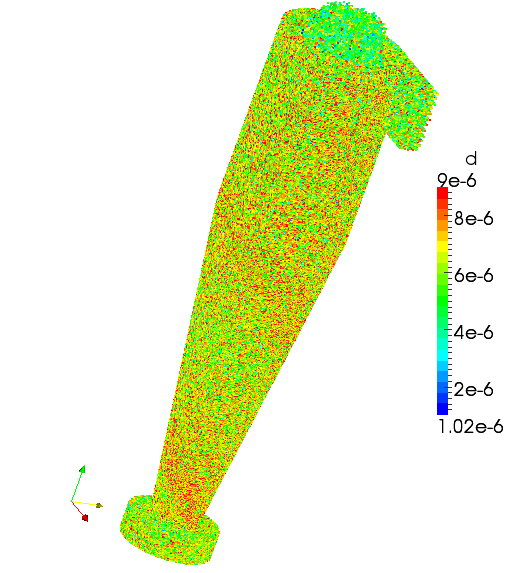
\includegraphics[scale=0.12]{parcelsCyclone4}\\
		\text{$d \sim 10^{-5}$, $U_{in} = 10m/s$}
	\end{minipage}
	\caption{Распределение дисперсных включений по диаметрам частиц в момент времени $t=1s$}
	\end{figure}
}
\frame{\frametitle{Сравнение результатов расчётов для эффективности циклонов с экспериментами Диргоу и Лейта}
	\begin{minipage}{\linewidth}
	\centering
	\begin{table}[h]
		\label{tableSolution}
		\begin{tabular}{|c|c|c|}
			\hline
			Параметры течения & $\eta$, численное исследование & $\eta$, эксперимент \\
			\hline
			$U_{in}=20m/s, d=5 \cdot 10^{-5}m$ & 100\% & 100\% \\
			\hline
			$U_{in}=20m/s, d=5 \cdot 10^{-6}m$ & 93\% & 90\%\\
			\hline
			$U_{in}=20m/s, d=5 \cdot 10^{-7}m$ & 27\% & 10\%\\
			\hline
			$U_{in}=15m/s, d=10^{-5}m$ & 80\% & 90\% \\
			\hline
			$U_{in}=10m/s, d=10^{-5}m$ & 72\% & 85\% \\
			\hline
			$U_{in}=5m/s, d=10^{-5}m$ & 75\% & 80\% \\
			\hline
		\end{tabular}
		\vspace{-1em}
	\end{table}
	\end{minipage}
	\vspace{1em}
	\hline
	\hline
	\begin{minipage}{\linewidth}
		\begin{figure}[h]
			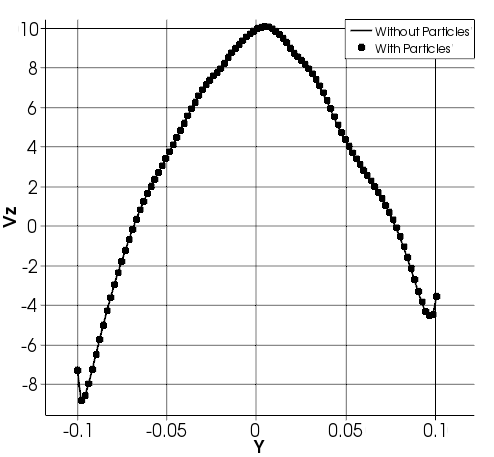
\includegraphics[scale=0.25]{parcelsInteraction}
			\caption{Распределение $V_z$ для задачи с частицами и без вдоль прямой $z=-1.5D$, $y=0$}
		\end{figure}
	\end{minipage}
}
\section*{}
\subsection{Заключение}
\frame{\frametitle{Заключение}
\begin{itemize}
\item В SST - модель турбулентности OpenFOAM был имплементирован поправочный коэффициент Шура-Спалларта для учёта влияния кривизны линий тока на турбулентные характеристики. Сравнение результатов расчётов с экспериментальными данными Монсона показало заметное улучшение по сравнению с немодифицированной SST - моделью.
\item Сравнение результатов расчётов циклона, выполненных при помощи модифицированного солвера OpenFOAM и Fluent показало отличное соответствие решений друг другу. Анализ влияния дисперсных включений на основной поток позволил заключить, что этим влиянием в исследуемой задаче, по большому счёту, можно пренебречь.

\item Проведено сравнение результатов расчётов с экспериментальными данными Диргоу и Лейта для степени очистки, которое показало хорошее согласие как с экспериментами, так и с теорией, которую эти эксперименты подтверждают.
\item Показана эффективность циклонов для очищения газа от твёрдых частиц диаметром $\sim 10^{-6}m$. Выявлено, что при уменьшении скорости течения, эффективность рассматриваемой конфигурации циклона заметно снижается. Такая же закономерность имеет место и при уменьшении диаметра частиц.
\item Выяснено, что для фильтрации частиц, диаметром меньше $\approx 10^{-7}m$, циклон непригоден так как степень очистки при этом становится меньше 30\%.
\end{itemize}
}
\end{document}
